\pagebreak
\section{Steering Order Test} %\label{put a label here and uncomment}
\textbf{Name: Group 510}\\
\textbf{Date: 11/11 - 2015}

\subsection{Purpose}
The purpose of the test is to find the needed order of the steering model, with a PWM signal as an input and the vehicle's angular velocity as an output.

\subsection{Theory}
As explained in \secref{sec:SteeringModel}, the input to the steering model is a PWM signal, which is applied to the servo motor. A specific PWM signal will make the servo rotate a specific amount. The servo controls the brakes and by rotating the servo, away from its middel position, the brakes will affect the wheels, on each side of the vehicle, differently, thus making the vehicle turn. These things are explained in more detail in \secref{sec:Vehicledescription}. The output from the test is the vehicle's angular velocity.

The objective is to get an angular velocity as an output with a PWM signal as an input. A test is performed where the vehicle drives in a circle, see \figref{fig:VehicletestSteeringCircle}. In the test it is not necessary for the vehicle to drive a complete circle, to get the needed parameters to calculate the angular velocity of the vehicle, only an arc of the circle is needed.

\begin{figure}[H]
  \centering
	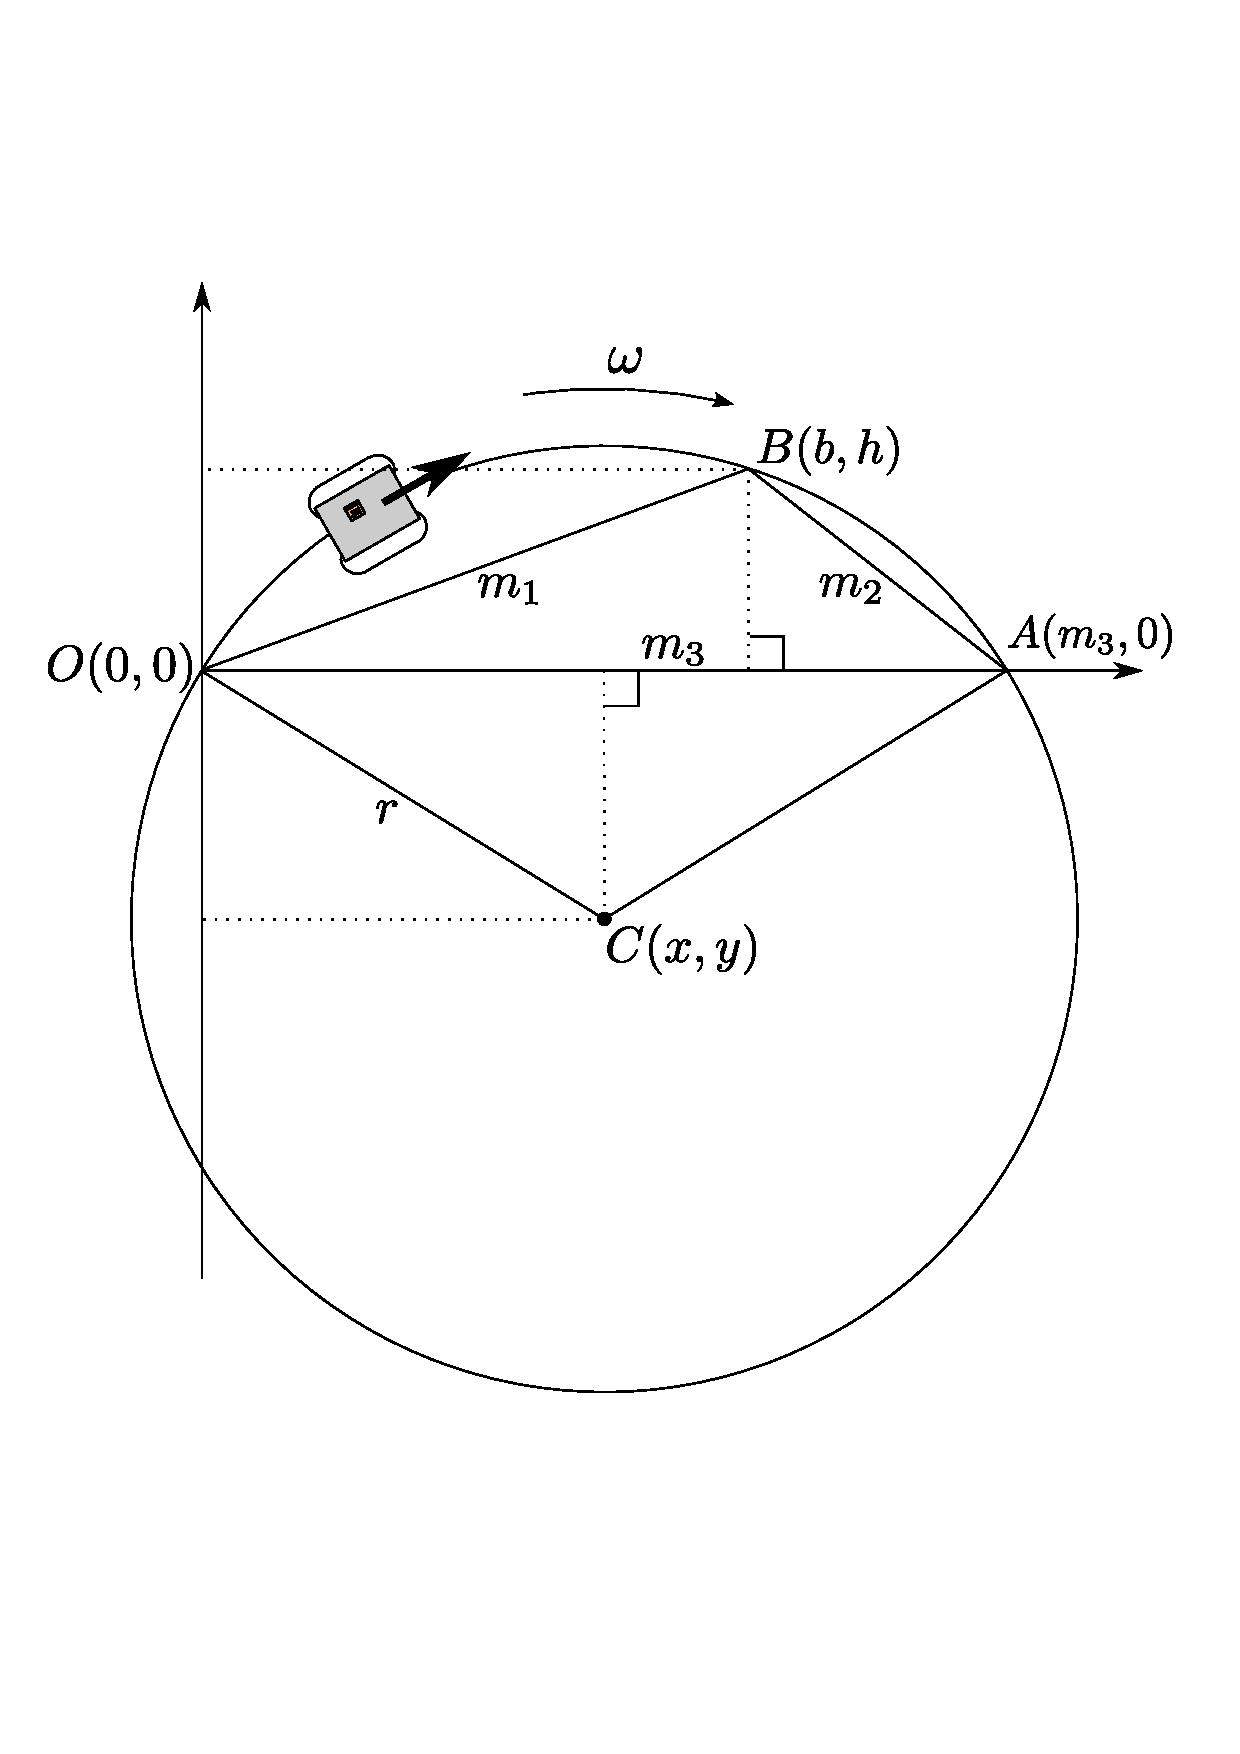
\includegraphics[scale=0.7]{figures/steeringmodelrotation.pdf}
	\caption{A diagram of the test setup}
	\label{fig:VehicletestSteeringCircle}
\end{figure}

To get the vehicle's angular velocity, the radius of the circle is needed. By using the illustration of the circle, in which the vehicle is driving, the equation for the radius can be derived.

\begin{flalign}
\eq{b}{\frac{m3^2 - m2^2 + m1^2}{2*m3}} \unit{\cdot}
\end{flalign}

\begin{flalign}
\eq{h}{\sqrt{(m1^2 - \frac{m1^2 - m2^2 + m3^2}{2*m3})^2}} \unit{\cdot}
\end{flalign}

\begin{flalign}
\eq{y}{\frac{b^2-b \cdot m3 + h^2}{2*m3}} \unit{\cdot}
\end{flalign}

\begin{flalign}
\eq{x}{\frac{m3}{2}} \unit{\cdot}
\end{flalign}

The y component of the C coordinate has been found, it is therefore possible to use Pythagoras theorem to find the equations for the circle's radius.

\begin{flalign}
\eq{r}{\sqrt{x^2+y^2}} \unit{\cdot}
\end{flalign}

By using the radius it is possible to create an expression for the angular velocity. It is assumed that the velocity is constant and the servo does not move after is has moved to a specific angle. by assuming these two things, the path which the vehicle will follow is the tangent of the circle. It is now possible to extract a equation for the vehicle's angular velocity.

\begin{flalign}
\eq{\omega}{\frac{v}{r}} \unit{rad \cdot s^{-1}}
\end{flalign}
\hspace{6mm} Where:\\
\begin{tabular}{p{1cm}lll}
& $\omega$ & is vehicle's angular velocity &\unitWh{rad \cdot s^{-1}}\\
& $v$   & is velocity of the vehicle &\unitWh{m \cdot s^{-1}}\\
\end{tabular}

The hall sensor is not used for finding points around the circle's arc, because it has been found faster to measure the points by hand. 

\todo{should the part with the hall sensor be in this subsection?}

\subsection{Setup}
\begin{figure}[H]
  \centering
	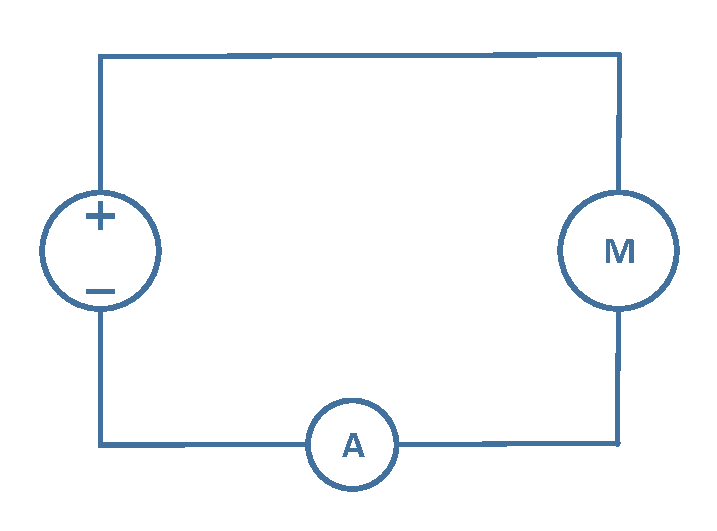
\includegraphics[scale=0.5]{figures/FrictionTest.pdf}
	\caption{A diagram of the test setup}
\end{figure}

\subsection{List of Equipment}

\begin{table}[H]
\begin{tabular}{|l|l|p{4cm}|}
\hline%------------------------------------------------------------------------------------
  \textbf{Instrument}                       &  \textbf{AAU-no.}  &  \textbf{Type}         \\
\hline%------------------------------------------------------------------------------------
  Multimeter                                &  60764             &  Fluke 189 true RMS    \\
\hline%------------------------------------------------------------------------------------
  Power Supply ($0 - 32$ V) ($0 - 10$ A)    &  77075             &  Ea - ps 7032 - 100    \\
\hline%------------------------------------------------------------------------------------
  Treadmill                                 &  75483             &  Rodby                 \\
\hline%------------------------------------------------------------------------------------
\end{tabular}
\end{table}

\subsection{Procedure}

\begin{enumerate}
  \item C
  \item P
  \item S
  \item A
  \item C
  \item R
  \item R
\end{enumerate}

\subsection{Results}


